%------------------------------------------------
\section{Введение}
%------------------------------------------------
\begin{frame}
 \frametitle{Актуальность}
 	\begin{itemize}
 		\item Коллайдерные эксперименты с поляризованными пучками;
 		\item Изучение Электрического Дипольного Момента когерентными пучками.
 	\end{itemize}

	 \begin{figure}
	 	\centering
	 	\includegraphics[width=0.24\linewidth]{"images/EDM CP"}
	 	\includegraphics[width=0.74\linewidth]{"images/EDM World"}
	 \end{figure}
	 

\end{frame}
%------------------------------------------------
\begin{frame}
	\frametitle{Цель и Задачи исследования}
	\textbf{Целью} данной диссертации является изучение особенностей динамики многозарядных тяжёлоионных и лёгких поляризованных пучков для проведения коллайдерных экспериментов в дуальной структуре, а также исследования электрического дипольного момента с использованием квази-замороженной концепции.\newline \newline
	Для достижения поставленной цели необходимо было решить следующие \textbf{задачи}:
	\begin{itemize}
		\item Расчёт времени внутрипучкового рассеяния и стохастического охлаждения;
		\item Моделирование магнитооптики с модулированной дисперсионной функцией;
		\item Проведение численного моделирования продольной динамики частиц;
		\item Изучение концепции «квази-замороженного» спина для исследования ЭДМ дейтрона и протона;
	\end{itemize}
\end{frame}
%------------------------------------------------
\begin{frame}
	\frametitle{Научная новизна}
	\begin{itemize}
		\item	Исследованы закономерности динамики многозарядных тяжёлых ионов и лёгких поляризованных частиц в дуальной магнитооптической структуре с учётом различий во внутрипучковом рассеянии и влияния критической энергии на устойчивость пучка;
		\vspace{1em}
		\item 	Предложен метод резонансной модуляции дисперсионной функции с применением дополнительного семейства квадрупольных линз, что позволило повысить критическую энергию и стабильность пучка в режиме ускорения лёгких частиц;
		\vspace{1em}
		\item	Приведены способы подавления дисперсии на краях поворотных арок в отсутствии регулярности, а также способы подавления нелинейных эффектов;
		\vspace{1em}
		\item 	Выполнено численное моделирование прохождения критической энергии с учётом высших порядков зависимости от импульсного разброса, а также влияния импедансов, что позволило количественно оценить влияние данных факторов на сохранение пучка;
	\end{itemize}
	
\end{frame}
%------------------------------------------------
\begin{frame}
	\frametitle{Научная новизна}
	\begin{itemize}
		\item	Исследована продольная динамика поляризованного пучка при нахождении вблизи и прохождении критической энергии методом скачка в гармоническом и барьерном ВЧ, что позволило количественно оценить стабильность пучка в различных режимах ускорения;
		\vspace{1em}
		\item	Предложено применение метода фильтров Вина для сохранения направления поляризации в пучках, что расширяет возможности по исследованию электрического дипольного момента и аксионоподобных частиц;
		\vspace{1em}
		\item	Рассмотрены вариации изучения ЭДМ дейтрона и протона в много-периодичных структурах с использованием электростатических дефлекторов или фильтров Вина;
	\end{itemize}
\end{frame}
%------------------------------------------------
\begin{frame}
	\frametitle{Практическая значимость}
	Исследования направлены на формирование полноценной физической программы по изучению динамики поляризованных пучков в комплексе Nuclotron-NICA. Применение изложенных в работе подходов возможно и на других похожих установках без потери общности.
\end{frame}
%------------------------------------------------
\begin{frame}
	\frametitle{Объект исследования}
	% TODO: \usepackage{graphicx} required
	\begin{figure}
		\centering
		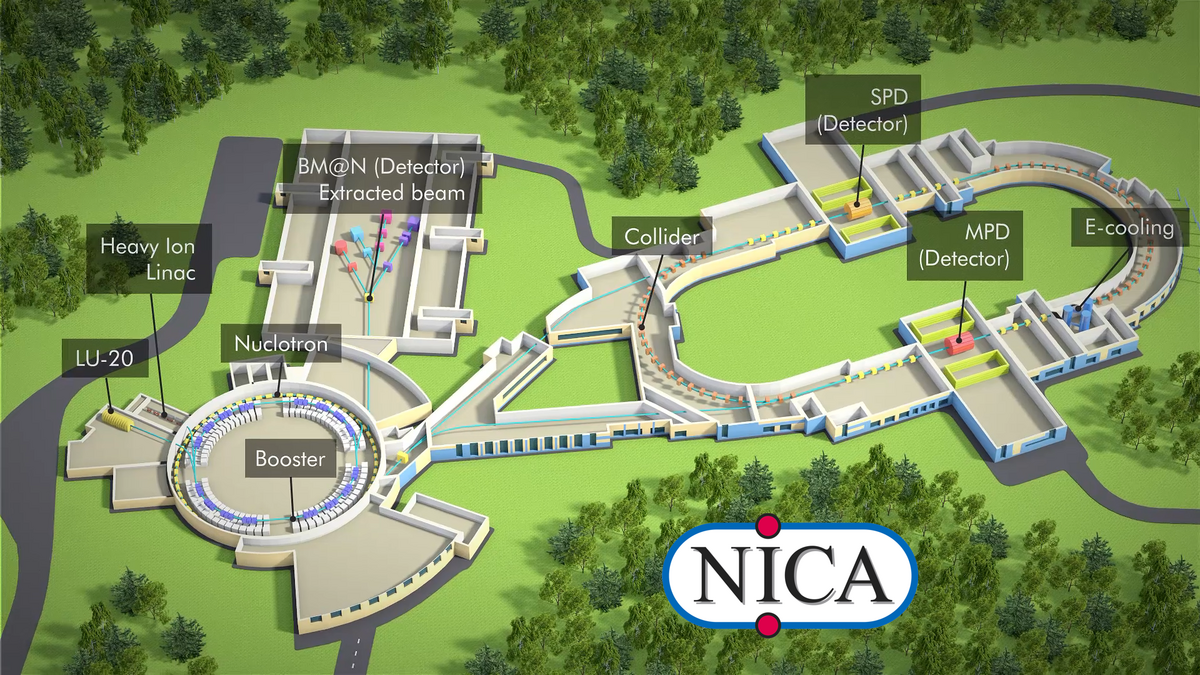
\includegraphics[width=0.6\linewidth]{images/NICA}
	\end{figure}
	
	Ускорительные и накопительные кольца, предназначенные для исследования поляризованных пучков заряженных частиц.
\end{frame}
%------------------------------------------------
\begin{frame}
	\frametitle{Методы исследования}
	\begin{enumerate}
		\item	Экспериментальные;
		\item	Аналитические и численные;
	\end{enumerate}
	\vspace{2em}
	\textbf{Экспериментальные} методы исследования заключаются в изучении динамики движения пучка с применением скачка критической энергии и без него.
	Соискатель лично участвовал в сеансе на синхротроне У-70 в г. Протвино, Россия в 2023 году.
	\vspace{1em}
	
	Математическое и компьютерное моделирование. Были использованы программы для расчёта поперечной динамики: MAD-X, OPTIM, BMAD, продольной динамики: BLonD; спин-орбитальной динамики: COSY Infinity.
\end{frame}
%------------------------------------------------
\begin{frame}
	\frametitle{Основные положения, выносимые на защиту}
	\begin{itemize}
		\item 	Основные свойства дуальной магнитооптической структуры для легких ядер и тяжелых частиц. Время жизни пучка с учетом вариации коэффициента проскальзывания в разных арках;
		\vspace{1em}
		\item	Учет влияния высших порядков разброса по импульсам и моделей продольных импедансов в окрестности критической энергии и сравнение с экспериментальными результатами, полученными на У-70;
		\vspace{1em}
		\item	Результаты моделирования прохождения ансамбля частиц через критическую энергию при различной форме ускоряющего потенциала с учетом ограничений по продольной микроволновой неустойчивости;
	\end{itemize}
\end{frame}
%------------------------------------------------
\begin{frame}
	\frametitle{Основные положения, выносимые на защиту}
	\begin{itemize}
		\item	Резонансная модуляция дисперсионной функции, метод вариации критической энергии. Результаты оптимизации при наличии отсутствующих магнитов;
		\vspace{1em}
		\item	Особенности поляризованных пучков, используемых для исследования ЭДМ в структурах с квази-замороженным спином на примере структуры Нуклотрон;
		\vspace{1em}
		\item	Метод фильтров Вина для сохранении направления поляризации на основе введения обводных каналов в структуре с квази-замороженным спином для выделения ЭДМ сигнала;
	\end{itemize}
\end{frame}
%------------------------------------------------